\chapter{App. methods: variational approach}
Fewest problems are exactly solved and we have to resort to approximate solution methods. The following approaches are available:
\begin{enumerate}
    \item[1.] Approximate the problem with an exactly solvable problem; this approach is particularly suitable for understanding the structure of the solution.
    \item[2.] Numerical solution via computer — this strategy provides precise numbers, but often does not help understanding, and should therefore only be used last.
    \item[3.] Variation Approach: Searching under a family of solutions that best understanding understanding of the solution structure and a good nose (for the approach) ahead, very elegant. 
    \item[4.] Perturbation calculation: Systematic improvement of the solution, good for developing the solution structure, can often provide exact figures. 
    \item[5.] Quasi-classic approximation: very physical, elegant, back-often-envelope arguments that reflect the relevant physics transparently 
\end{enumerate}
Point {\color{red}1} was worked out in the previous chapters with some examples. Point {\color{red}2} is dealt with in other lectures. We start with point {\color{red}3}, the variation approach. We will discuss the disturbance calculation in Chapter 9, and we will work on the quasi-classical approximation in Chapter 10.\par
The variation calculation is based on the Rayleigh-Ritz (RR) variation principle: Let $\Psi$ be a state function, $H$ a Hamiltonian with ground state energy $E_0$, then
%公式 1
\begin{equation}
    \frac{\langle\Psi|H| \Psi\rangle}{\langle\Psi | \Psi\rangle} \geq E_{0}
    \end{equation}
because with the own base $\varphi_n$ to $H$
%公式 2
\begin{equation}
\begin{aligned}\langle\Psi|H| \Psi\rangle &=\sum_{n}\left\langle\Psi | \varphi_{n}\right\rangle \underbrace{\left\langle\varphi_{n}|H| \varphi_{n}\right\rangle}_{E_{n} \geq E_{0}}\left\langle\left\langle p_{n} | \Psi\right\rangle\right.\\ & \geq E_{0} \sum_{n}\left|\left\langle\Psi | \varphi_{n}\right\rangle\right|^{2} \\ &=E_{0}\langle\Psi | \Psi\rangle \end{aligned}
\end{equation}
This equation allows us to get an upper bound on the ground state energy (and the ground wave function $\Psi_0$): Take any $\Psi$, then $\langle \Psi|H|\Psi\rangle/\langle\Psi|\Psi\rangle$ gives an upper bound on ¨ $E_0$. We can write $\Psi$ as
%公式 3
\begin{equation}
    \Psi=\alpha \Psi_{0}+\beta \Psi_{0}^{\perp}
    \end{equation}
where $\Psi_0^{\perp}\perp\Psi_0$. It is $\langle\Psi|\Psi\rangle = |\alpha|^2+|\beta|^2$, so our $\Psi$ the better the smaller the correction $\Psi_0^{\perp}$: the correct ‘direction’ is to be found in Hilbert space $H$.\par
The RR principle also allows excited states to be estimated: If $\Psi_0$ is known, then the best function $\Psi-\langle\Psi_0|\Psi\rangle\Psi_0$ (with the lowest energy) gives the first excited state. The principle can be iterated for undegenerate problems:
The optimization in
%公式
$$
    \mathcal{H}_{\perp}^{N}=\left\{\Psi-\sum_{n=0}^{N-1}\left\langle\Psi_{n} | \Psi\right\rangle \Psi_{n} | \Psi_{n}=\mathrm{E} \mathrm{V} \text { to the } N-1 \text { deepest EW } E_{n}\right\}
$$
gives $E_N$ and $\Psi_N$. In particular, one finds EN from the diagonalization of the matrix $\langle\Psi_k|H|\Psi_m\rangle$, with $\{\Psi_k\}$ a basis in $\mathcal{H}_N$; $E_N$ is then the smallest representative of the largest eigenvalue $\lambda$ in $\mathcal{H}_N$ with variation of $\mathcal{H}_N$. Or simply expressed in a formula, $E_N=\operatorname{inf}_{\mathcal{H}_N}\{\operatorname{max}_{\lambda}[EW(\langle\Psi_k|H|\Psi_m\rangle|\Psi_k,\Psi_m\in\mathcal{H}_N,\operatorname{dim}\mathcal{H}_N=N)]\}$. Symmetries can also be exploited: Let $SO (3)$ be a symmetry of $H$. Applying the RR principle in the subspaces $\mathcal{H}_l$ to the angular momentum $L^2 = \hbar^2l (l + 1)$ results in a barrier for the smallest energy with angular momentum $\hbar^2l (l + 1)$.
\par
We can also get \textit{lower} bounds, but this is generally much more difficult. A luck case is when ¨ $H = H_0 + V$ can be dismantled with $V \geq 0$. Let ΨG be the ground state of $H$, then

%公式 4
\begin{equation}
\begin{aligned} E_{G} &=\left\langle\Psi_{G}|H| \Psi_{G}\right\rangle \\ &=\underbrace{\left\langle\Psi_{G}\left|H_{0}\right| \Psi_{G}\right\rangle}_{\geq E_{0}}+\underbrace{\left\langle\Psi|V| \Psi_{G}\right\rangle}_{\geq 0} \geq E_{0} \end{aligned}
\end{equation}
In (8.4) we used that the ground state for $H_0$ with energy $E_0$ is generally given by $\Psi_0\neq\Psi_G$, and thus $\langle\Psi_G|H_0|\Psi_G\rangle\geq\langle\Psi_0|H_0|\Psi_0\rangle=E_0$. In the following we look at an example.

\section{Basic state of the He-atom}
The helium atom consists of a nucleus with two electrons,
%公式 5
\begin{equation}
    \mathrm{He}=\underbrace{2 \mathrm{p}+2 \mathrm{n}}_{+2 e \text { charge }}+2 e^{-}
    \end{equation}
We only consider the electronic degrees of freedom and describe the two-particle problem of the electrons in the field of the nucleus. The Hamilton operator in the location display is
%公式 6
\begin{equation}
    H=-\frac{\hbar^{2}}{2 m}\left(\vec{\nabla}_{1}^{2}+\vec{\nabla}_{2}^{2}\right)-2 e^{2}\left(\frac{1}{r_{1}}+\frac{1}{r_{2}}\right)+\frac{e^{2}}{\left|\vec{r}_{1}-\vec{r}_{2}\right|}
    \end{equation}
We know the ground state for an H-atom ($a_B=\hbar^2/m_ee^2$ the Bohr radius)
%公式 7
\begin{equation}
    \Psi_{0}=\left(\frac{1}{\pi a_{B}^{3}}\right)^{1 / 2} \exp \left(-\frac{r}{a_{B}}\right)
    \end{equation}
and use it to construct the variation approach
%公式 8
\begin{equation}
    \Psi\left(\vec{r}_{1}, \vec{r}_{2}\right)=\frac{\alpha^{3}}{\pi a_{B}^{3}} \exp \left[-\alpha\left(r_{1}+r_{2}\right) / a_{B}\right]
    \end{equation}
We will see later that this approach is compatible with the Pauli principle: the exact ground state of the He atom has the structure
%公式 9
\begin{equation}
    \Psi\left(\vec{r}_{1}, s_{1} ; \vec{r}_{2}, s_{2}\right)=\Psi_{\mathrm{Sym}}^{\mathrm{Bahn}}\left(\vec{r}_{1}, \vec{r}_{2}\right) \otimes \Psi_{\text {Antisym }}^{\mathrm{Spin}}\left(s_{1}, s_{2}\right)
    \end{equation}
where $s_i$ are the spin quantum numbers and ‘sym / antisym’ indicates the symmetry of the function $\Psi$ while swapping the variables. (8.8) has the right symmetry.\par
We have to calculate the expected value $\langle\Psi|H|\Psi\rangle$. For H-atoms, $E_0^{kin}=e^2/2a_B$ and $E^{pot} = -e^2 / a_B$; because of the changed length $r \rightarrow\alpha r$ in (8.8) these energies are scaled according to
%公式 10
\begin{equation}
    E^{\mathrm{kin}}=2 \cdot \frac{e^{2} \alpha^{2}}{2 a_{B}}, \quad E^{\mathrm{pot}}=-2 \cdot \frac{2 e^{2} \alpha}{a_{B}}
    \end{equation}
where the doubling takes into account the presence of two electrons (the additional factor two in $E^{pot}$ takes into account the doubled charge in the He nucleus). The calculation of the interaction energy
%公式 11
\begin{equation}
    E^{\mathrm{WW}}=\left(\frac{\alpha^{3}}{\pi a_{B}^{3}}\right)^{2} e^{2} \iint \mathrm{d}^{3} r_{1} \mathrm{d}^{3} r_{2} \frac{\exp \left[-2 \alpha\left(r_{1}+r_{2}\right) / a_{B}\right]}{\left|\vec{r}_{1}-\vec{r}_{2}\right|}
    \end{equation}
involves the following transformations: we use that $1 / r$ is the Green's function of the Laplace operator,
%公式 12
\begin{equation}
    \Delta(1 / r)=-4 \pi \delta^{3}(\vec{r}), \quad \mathcal{F}[1 / r]=4 \pi / k^{2}
    \end{equation}
and represent the coulom energy in the$\vec{k}$-space by the integral
%公式
$$
    \frac{e^{2}}{\left|\vec{r}_{1}-\vec{r}_{2}\right|}=4 \pi e^{2} \int \frac{d^{3} k}{(2 \pi)^{3}} \frac{1}{k^{2}} \mathrm{e}^{i \vec{k} \cdot\left(\vec{r}_{1}-\vec{r}_{2}\right)}
$$
The integration over the location coordinate $\vec{r}=\vec{r}_1$ results (likewise with $\vec{r}_2$)
%公式 13
\begin{equation}
\begin{aligned} \int d^{3} r \mathrm{e}^{i \vec{k} \cdot \vec{r}-2 \alpha r / a_{B}} &=\frac{4 \pi}{k} \int_{0}^{\infty} d r \operatorname{Im}\left[r \mathrm{e}^{i k r-2 \alpha r / a_{B}}\right] \\ &=\frac{16 \pi \alpha / a_{B}}{\left(k^{2}+4 \alpha^{2} / a_{B}^{2}\right)^{2}} \end{aligned}
\end{equation}
The remaining integration over $\vec{k}$ gives us the interaction energy
%公式 14
\begin{equation}
    E^{\mathrm{WW}}=\frac{5 \alpha}{8} \frac{e^{2}}{a_{B}}
    \end{equation}
This gives the total energy to
%公式 15
\begin{equation}
    \langle H\rangle(\alpha)=\alpha^{2} \frac{e^{2}}{a_{B}}-4 \alpha \frac{e^{2}}{a_{B}}+\frac{5}{8} \alpha \frac{e^{2}}{a_{B}}
    \end{equation}
it is minimized by $\alpha = 27/16$ and gives the following estimate for the ground state energy,
%公式 16
\begin{equation}
    E_{0} \leq-\left(\frac{27}{16}\right)^{2} \frac{e^{2}}{a_{B}} \approx-2.85 e^{2} / a_{B}
    \end{equation}
This result is very close to the measured value $E_0 \approx -2.904 e^2 / a_B$. Interpretation: Trivially we could expect α = 2 since the charge is $Z = 2$. However, we find the reduced value $\alpha = 27/16 \leq 2$: each $e^-$ shields the core for the other ¨ $e^-$ with an effective charge 5/16, as shown in sketch {\color{red}8.1}.
\begin{figure}[ht]
    \begin{minipage}{0.5\textwidth}
        \centering
        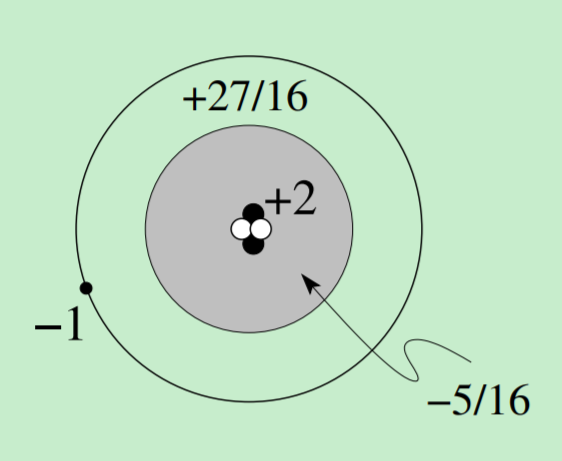
\includegraphics[scale=1]{8_1.PNG}
    \end{minipage}
    \begin{minipage}{0.5\textwidth}
        \captionsetup{font={Large}}
        \caption{Shielding: the second electron (charge -1) moves in the middle field of the core (charge +2) and the first electron (effective shield charge -5/16); on the second electron thus acts an effective charge 27/16.}
    \end{minipage}
\end{figure}